\documentclass[journal]{IEEEtran}

\usepackage[T1]{fontenc}
\usepackage[utf8]{inputenc}
\usepackage{amsmath,amssymb}
\usepackage{graphicx}
\usepackage{textcomp}
\usepackage{xcolor}
\usepackage[noend]{algpseudocode}
\usepackage{algorithm}
\usepackage{xeCJK}
\setCJKmainfont{Heiti SC}

\graphicspath{{code/figures/}}

\newtheorem{proposition}{命题}
\newtheorem{lemma}{引理}

\begin{document}

\title{交互动力学：面向人形机器人的物理交互推理层\\[2pt]\large（中文译本）}

\author{Anonymous Author(s)%
\thanks{本文为英文原稿的中文译本，内容以英文原稿为准。原稿提交用于双盲评审；为保持匿名，译本同样不附带作者身份信息。}%
}

\markboth{提交用于双盲评审}{Anonymous Author(s)：交互动力学——面向人形机器人的物理交互推理层}

\maketitle

\begin{abstract}
行走机器人必须应对性质迥异的物理接触。一次短暂的推力会注入动量，最好的应对方式是朝跌倒方向迈步以捕获该动量；而一个持续力——例如倚靠或负载——则必须通过反向迈步来抵抗。这两种响应符号相反，但仅凭质心（CoM）运动学量无法在线区分这两种情形，因为一次已恢复的推力扰动和一个持续站立的外力会留下相同的侧向偏移。真正将二者区分开的，是外力是否仍在作用——而这并不是一个运动学量。我们从质心水平方向的动量残差中估计外力，并据此选择响应方式。由此得到的交互动力学（Interaction Dynamics）层置于一个冻结的强化学习行走策略与机器人之间，对策略的速度指令施加偏置修正。一个置信门仅在估计的外力超出其自身实测噪声本底时才使该层介入，而一个持续性计时器则在预测性捕获指令与积分保持之间进行混合。在仿真的 Unitree G1 上，该层将 280~N 单支撑推力下的跌倒次数从 24/40 降至 2/40（McNemar 检验 $p<10^{-4}$，且没有任何配对试验变差），并将 8~N 持续外力下的侧向漂移保持在 13~mm，与专用保持控制器的 12~mm 相当，同时名义行走性能不受影响。我们将该层视为位于运动规划之下、全身控制之上的一个快速、短时域的物理交互接口。
\end{abstract}

\begin{IEEEkeywords}
交互动力学、外力估计、人形机器人步行、推力恢复、物理人机交互、基于模型的 Physical AI、交互模式仲裁、基于置信度的模式选择。
\end{IEEEkeywords}

\section{引言}
\label{sec:intro}

现实物理世界中的腿式机器人持续受到\emph{外部交互}的作用：手会推它，工具与负载会加载于它，地形也会施加与运动规划假设不同的接触力。这种交互具有异质性。人群中的一次推搡是一次\textbf{瞬态冲击}——一个短暂的高幅力，注入动量后随即消失。有人倚靠在机器人上、风载荷、或持续的接触，则是一个\textbf{持续力}——一个必须被持续抵抗的低幅稳态力。这两种模式不仅仅是幅值不同，它们要求\emph{相反}的控制动作。要从一次瞬态推力扰动中恢复，双足机器人必须朝跌倒方向迈步，使一只脚落在正在加速的质心下方（捕获步）。而要在持续力下保持位置，它则必须反向倾斜并迈步以抵抗该力。把瞬态响应用于持续力会放大漂移；把持续响应用于瞬态推力则无法遏制住动量。

本文提出三项观察，它们共同促使我们在控制栈中引入一个新的层。

\textbf{观察 1（判别问题）。} 正确的交互模式无法仅凭质心运动学量推断出来。一次瞬态推力和一个持续力可能留下\emph{相同}的持续侧向位移：推力过后，双足机器人会在一个平移后的位置上恢复平衡，因此其质心误差会无限期地保持非零——仅凭位置和速度，这与一个持续站立的外力是无法区分的。真正具有区分性的信息是\emph{外力是否仍在作用}，而这不是一个运动学量。

\textbf{观察 2（表示形式）。} 尽管存在这种异质性，所有外部交互都共享同一种表示形式。在选定的任务坐标下，经过名义动力学补偿后，跟踪误差服从一个固定的双重积分器模型，其驱动项是单一的\emph{交互残差} $d_{\rm eff}$，它汇聚了外力、实现误差与模型失配。该模型在构型和接触模式变化下保持不变：交互由此成为一个共享模型上的\emph{预测状态}，而不是一个需要针对每种接触重新建模的属性。

\textbf{观察 3（时间尺度）。} 物理交互控制与感知工作在不同的时间尺度上，解决的也是不同的问题。感知与规划在数十到数百毫秒的尺度上对世界和任务进行推理，例如识别地形、预测人的意图、或重新规划落脚点。对外力的响应等不到那一层循环完成：响应必须是即时的，而且只需要交互的估计量，不需要世界模型。这就要求在规划之下、执行器之上设置一个短时间尺度的层，其职责是在较慢的循环更新期间管理物理交互。这一分工正是一个基于模型的 Physical AI 技术栈的组织方式：感知与规划对世界进行推理，而一个快速的交互层则直接处理物理交互本身；二者是互补而非竞争关系。

这使得该控制问题成为一个模式选择问题，而不是力调节问题。经典的交互控制器，例如阻抗与导纳方案，假设交互始终以单一形式存在，并只调节其幅值。而在这里，模式本身是未知的，必须在线推断：该层必须先判断是否存在外部交互，再判断属于哪种模式，然后才能采取行动。正是外力估计使这两个判断成为可能，而这恰恰是质心运动学量所缺少的信息。

我们将这一层称为\textbf{交互动力学（Interaction Dynamics）}。图~\ref{fig:arch} 展示了它在一个基于模型的 Physical AI 层级结构中的位置。

\begin{figure}[t]
\centering
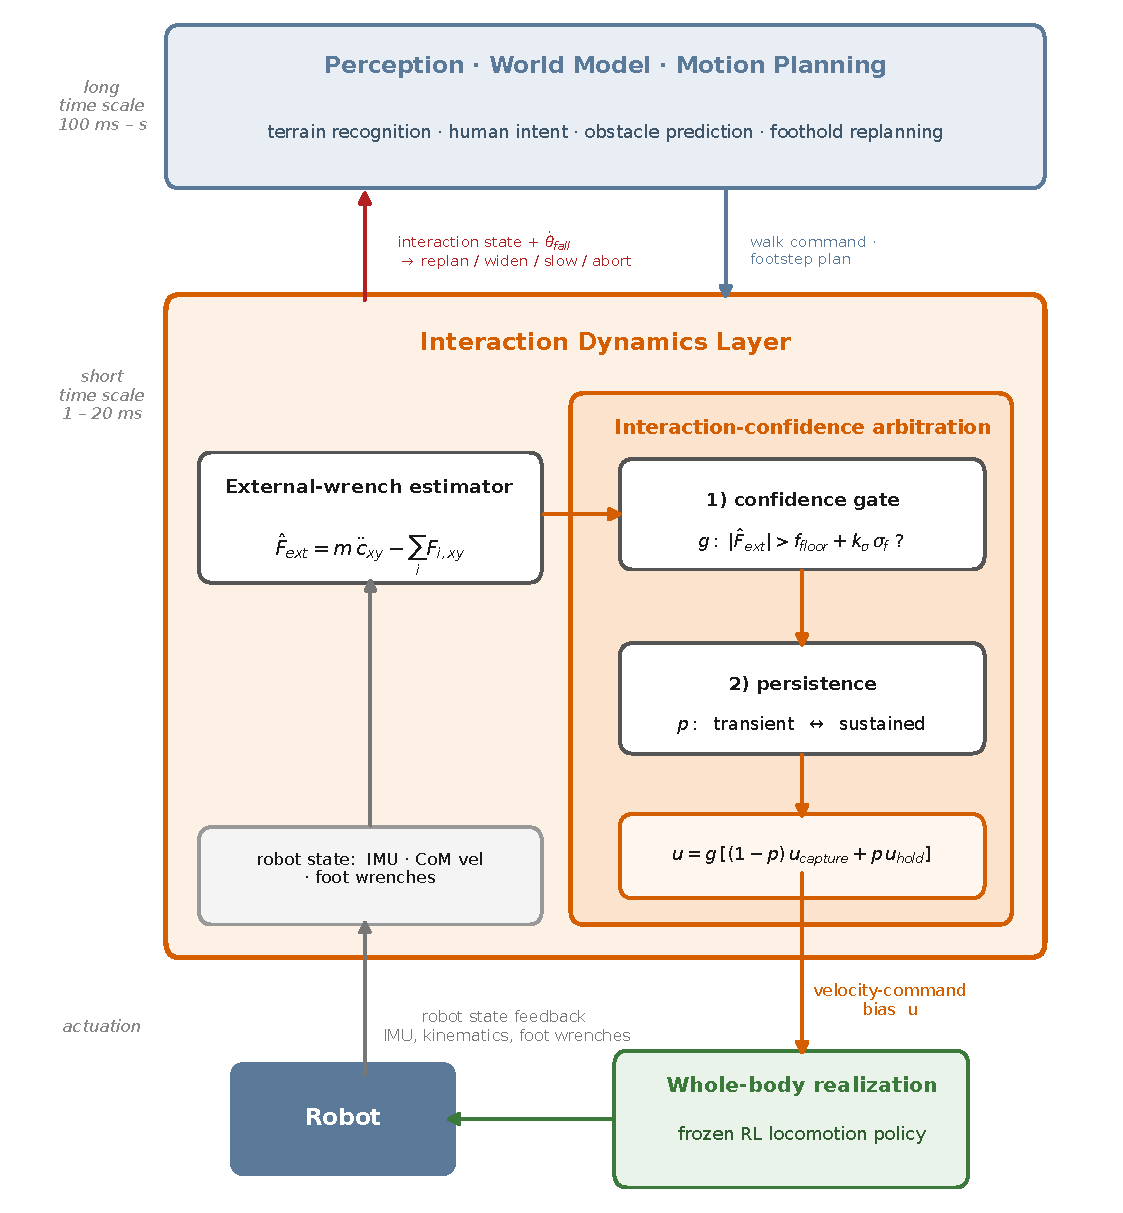
\includegraphics[width=\columnwidth]{architecture}
\caption{交互动力学作为规划与全身实现层之间的快速物理交互层。它估计外力，通过一个两级置信度机制在捕获与保持之间进行仲裁，并调制冻结策略的行走指令；跌倒速率线索 $\dot\theta_{\rm fall}$ 通过一个\emph{被提议但尚未评估}的规划器接口向上返回。}
\label{fig:arch}
\end{figure}

该层通过三个步骤来完成这一决策。它估计外力及其已持续的时间，判断是否存在真实的交互、以及该交互是瞬态还是持续，然后施加相应的修正：交由策略处理、捕获、或保持。因此，估计器、置信门与持续性分类器是同一条流水线的组成部分，而不是彼此独立添加的模块。第~\ref{sec:rep}节建立表示形式，第~\ref{sec:est}节给出估计器，第~\ref{sec:control}节给出门控与控制；第~\ref{sec:val}节对结果进行评估。

该层并不取代感知或规划，它只是在新规划尚未生成的这段时间内提供稳定性。当扰动超出该层的权限范围时，它所暴露出的状态——例如一个跌倒角，其变化率表明稳定权限即将耗尽——正是上层用来判断是否需要拓宽支撑姿态、减速、重新规划落脚点或放弃任务的信号。

为了让本文的贡献聚焦于交互本身而非步行控制本身，我们刻意将步行控制作为一个\textbf{冻结的验证平台}：我们采用一个现成的、针对 Unitree G1 预训练好的强化学习行走策略~\cite{r16}，将其冻结，并且在任何交互实验中都不对其进行调参。交互层置于其上，对该策略的行走指令进行调制。一个自然的替代方案——像经典交互控制那样，通过一个全身逆动力学/接触 QP 来实现交互修正——结果反而会使一个强健的学习策略\emph{失稳}，因为该策略的平衡是其自身控制律的一个闭环属性；我们将此作为一个负面结果予以报告，它正是促使我们采用指令调制耦合方式的原因。

本文做出四项贡献。
\begin{enumerate}
\item \emph{问题建模。} 我们证明，在共享的步行控制接口下，瞬态交互与持续交互要求相反的指令空间恢复动作，且仅凭质心运动学量无法在线区分两者。
\item \emph{方法。} 一种基于外力门控的持续性仲裁机制，它在预测性捕获指令与积分保持之间进行混合，并通过冻结的学习策略自身的速度指令接口对其进行驱动。源自质心线性动量残差的外力估计是使能信号，而固定的、构型不变的模型（引理~\ref{lem:model}，改编自~\cite{r1}）则是其基底。
\item \emph{性质。} 捕获路径透明性——该层在未介入时退化为冻结策略本身，且无法触发捕获失控；以及在有界估计误差下的有界增强指令（命题~\ref{prop:gate}–\ref{prop:bounded}）。
\item \emph{评估。} 在 Unitree G1 上开展的一项配对人形机器人研究，包含专用控制器、仅质心和 oracle 消融实验、统计学意义上的推力与持续力测试、传感鲁棒性扫描，以及一种被置信门解决的捕获放大失效模式。
\end{enumerate}

\section{相关工作}
\label{sec:related}

\textbf{步行控制。} 凸 MPC~\cite{r2,r3,r13}、全身逆动力学与分层 QP~\cite{r4,r5,r7,r9}，以及统一的全身 MPC~\cite{r10}，都将接触与支撑嵌入到预测模型之中。我们则不同：我们预测一个固定的双重积分器任务模型，并在一个冻结的控制器之上添加一个薄层。

\textbf{推力恢复与反应式迈步。} 从推搡中恢复，经典上是通过捕获点与运动的发散分量（divergent component of motion）来实现的~\cite{r20,r21}，并辅以反应式迈步来遏制动量~\cite{r22}。这些方法针对的是瞬态情形，且都假设存在一个基于模型的迈步控制器。我们对瞬态情形保留了这种捕获行为，另外增加了一个显式的持续力模式，在线地在二者之间进行选择，并通过一个学习策略自身的指令接口来执行，而不是依赖专用的迈步控制器。

\textbf{外力与动量观测器。} 借助广义动量观测器，无需力传感器也能估计外力~\cite{r14,r15}，该方法已用于机械臂、以及最近的人形机器人的碰撞检测与反应~\cite{r25}。我们使用质心的\emph{线性}动量残差，但并非将其作为碰撞标志，而是作为驱动模式选择的置信度与持续性信号。

\textbf{在冻结策略上分层。} 在一个固定的学习策略上添加基于模型的修正，这与残差强化学习~\cite{r23}以及监督式与多模型控制相关，其中由更高层的逻辑在多个控制器之间切换或混合~\cite{r24}。在这个意义上，我们的层是一种监督式仲裁：一个置信门与一个持续性分类器在不重新训练策略的前提下，混合两个手工设计的修正量。

\textbf{交互控制与本文定位。} 阻抗与导纳控制~\cite{r6,r11,r12}假设交互始终以单一形式存在，并只调节其幅值；而我们把当前存在的是哪种模式本身当作未知量来处理。固定模型表示及其针对固定基座接触的无偏调节方法最初在~\cite{r1}中提出，我们将其推广到浮动基座上。外力估计、置信度门控、基于持续性的混合、以及指令空间增强，这些要素本身都并非全新；本文的贡献在于将它们组合成一个交互层，在一个冻结的人形步行器上于瞬态捕获与持续保持之间进行仲裁。

\section{交互动力学：表示形式}
\label{sec:rep}

\subsection{浮动基座模型与任务残差}
\label{sec:rep-model}

记广义坐标为 $q=[q_b^\top,q_j^\top]^\top$（浮动基座与主动关节），系统动力学为
\begin{equation}
M(q)\ddot q+h(q,\dot q)=S^\top\tau+J_c^\top\lambda+w_{\rm ext},
\label{eq:dyn}
\end{equation}
其中 $\lambda$ 为接触力旋量，$w_{\rm ext}$ 为外部交互。设 $y$ 收集选定的任务坐标（此处为平面内的质心位置），$e=y-y_d$ 为相对名义规划的跟踪误差。在任务惯量良态且存在名义前馈的条件下，实际实现的误差服从\textbf{典范交互模型}
\begin{equation}
\ddot e=a_e+d_{\rm eff},\qquad d_{\rm eff}=d_{\rm int}+d_{\rm real}+d_{\rm mod},
\label{eq:model}
\end{equation}
其中 $a_e$ 为所指令的任务加速度修正量，$d_{\rm int}=M_p^{-1}F^{\rm ext}$ 为外部交互在任务加速度上的效应，$d_{\rm real}$ 为实现差异，$d_{\rm mod}$ 为模型残差。

\begin{lemma}[固定的请求任务预测器]
\label{lem:model}
对于一个相对阶为 $r$、且其请求坐标在一组接触模式上保持固定的任务而言，式~\eqref{eq:model} 的精确零阶保持（ZOH）转移矩阵对是阶数为 $r$ 的积分链矩阵对 $(A_d,B_d)$，它仅是采样周期与 $r$ 的函数。机器人力学特性、接触几何与环境仅通过 $d_{\rm eff}$ 与可行指令集进入模型，从不进入 $(A_d,B_d)$。一次接触切换会改变残差与恢复映射，但预测矩阵保持不变。（在任务惯量良态且名义前馈精确的条件下；该积分链结果的推导如~\cite{r1}中所示，此处将其推广到浮动基座。）
\end{lemma}

\emph{为何固定模型已经足够。} 预测矩阵对 $(A_d,B_d)$ 描述的仅仅是一个任务坐标及其变化率在一次采样内、在指令任务加速度作用下如何演化——这是纯粹的积分链运动学，对机器人本身一无所知。所有\emph{真正}与机器人和接触相关的量——质量矩阵、科氏力与重力项、接触雅可比、以及外部力旋量——都只通过实际产生的加速度进入模型，也就是通过 $d_{\rm eff}$ 与可行指令集进入。因此，改变机器人、地形或接触状态，改变的是\emph{需要什么样的修正、以及该修正是否可达}，而不是把指令映射为运动的那个积分器本身。这正是为什么单一的归一化模型能够承载原本各自需要独立、依赖接触的模型才能描述的诸多交互。

\emph{该表示形式的精确程度如何？} 在引理~\ref{lem:model}的假设下，即名义动力学补偿与任务空间投影成立时，模型 $\ddot e = a_e + d_{\rm eff}$ 是\textbf{精确的}，而不是一种线性化：它是把 $d_{\rm eff}$ \emph{定义}为动力学实际产生的、超出 $a_e$ 的那部分加速度。近似仅通过不完美的补偿和未建模动力学引入，且不会污染预测矩阵；它被吸收进模型残差项 $d_{\rm mod}\subseteq d_{\rm eff}$ 中，估计器与控制器对它的处理方式，与处理外力完全一致。因此，在所述输入定义下，该积分器结构是一个精确的坐标恒等式；然而，它在\emph{预测}方面的有效性是有条件的——取决于残差在控制时域内是可观测且足够持续的，也取决于策略介导的指令映射（第~\ref{sec:realize}节）在局部上保持一致。一个幅值很大或快速变化的 $d_{\rm mod}$ 不会破坏这一恒等式，但可能使固定模型在预测上失去信息量。

因此，交互是共享固定模型上的一个\emph{预测状态}。这里有一个区分很重要：对于\emph{控制}而言，捕获律抵消的是聚合残差，无需将其拆分为各部分；而对于\emph{模式分类}而言，则必须把力这一分量单独分离出来。将 $d_{\rm eff}$ 写作 $d_{\rm eff}=\underbrace{m^{-1}F_{\rm ext}}_{d_{\rm int}}+(d_{\rm real}+d_{\rm mod})$ 后，瞬态与持续之间的判断只依赖 $d_{\rm int}$ 本身——一个聚合的加速度残差无法把一个持续的外力，与一个持续的实现偏差或模型偏置区分开来——而第~\ref{sec:est}节中的线性动量估计器恰好恢复出这一分量，$\hat d_{\rm int}=m^{-1}\hat F_{{\rm ext},xy}$。这一表示形式是一种建模上的\emph{选择}，而且是一种可证伪的选择：只有当抵消性修正 $a_e=-d_{\rm eff}$ 是可行且可实现的时候，任务才会被调节到零稳态误差；超出指令权限范围的外力，会表现为一个未被抑制的残差或平衡的丧失，而不是一种可自由重新贴标签的现象。

\subsection{瞬态/持续二分法}
\label{sec:dichotomy}

残差模型~\eqref{eq:model} 在 $d_{\rm eff}$ 上是对称的，但\emph{恰当的修正}并不对称（图~\ref{fig:dichotomy}）。考虑一个侧向扰动。

\textbf{瞬态冲击。} 外力短暂作用，注入质心速度；此后 $d_{\rm int}\!\to\!0$，但动量仍然存在。稳定化动作是命令行走层朝误差速度\emph{的方向}迈步，将摆动腿落在正在跌落的质心下方（捕获）。有效修正的符号是 $+\dot e$。

\textbf{持续力。} 外力持续存在；若不采取动作，质心会持续漂移。稳定化动作是命令\emph{反向}于误差，并加入一个积分项以实现减偏抑制。符号是 $-e-\!\int\! e$。

这两者是相反的——更准确地说，在本文所评估的速度指令接口下，有效的指令空间恢复动作符号相反（这一点对踝/髋策略，或纯力调节目标而言未必成立）。此外（观察 1），$e$ 与 $\dot e$ 无法区分二者：一次瞬态推力会留下一个持久的位置偏移（在一个平移后的姿态上恢复），因此对\emph{偏差}本身做持续性检验会出现误判。真正具有区分性的变量是外力本身——它在持续力下始终存在，而在瞬态冲击下（脉冲过后）则不再存在——即便此时质心仍在恢复过程中。第~\ref{sec:est}–\ref{sec:control}节正是围绕这一变量来构建估计器与仲裁机制的。

\begin{figure}[t]
\centering
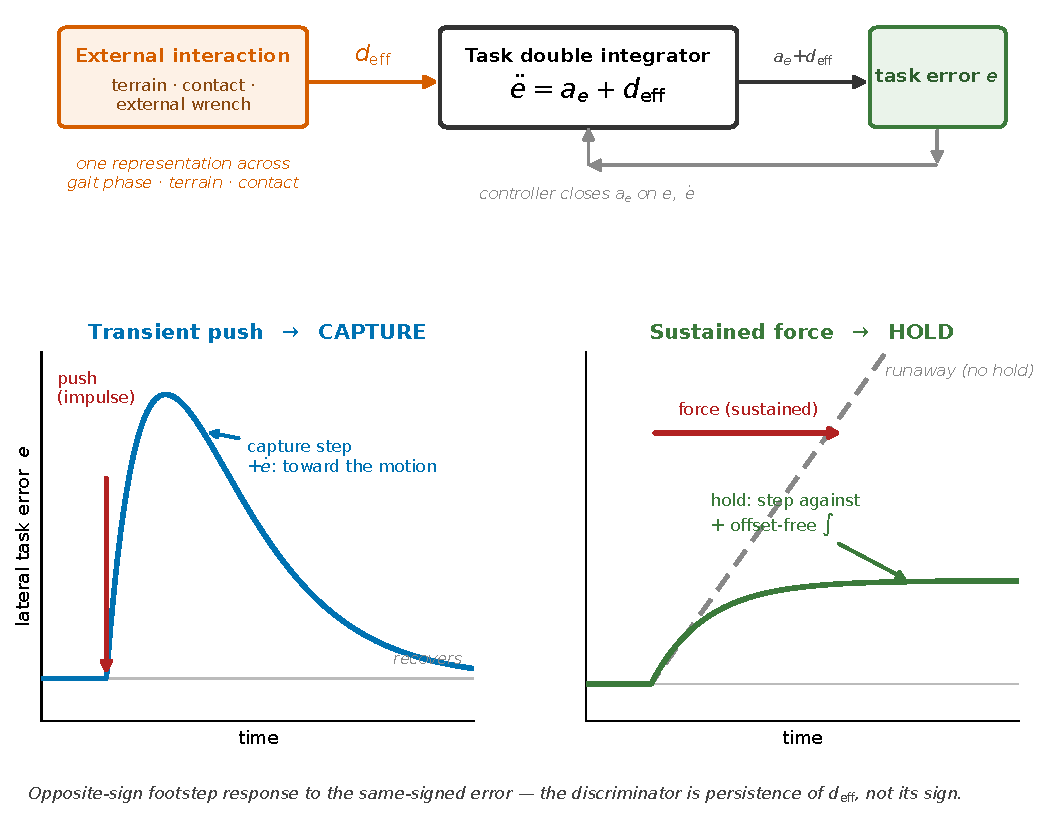
\includegraphics[width=\columnwidth]{model_dichotomy}
\caption{表示形式与二分法。\emph{上：}交互被汇聚为固定双重积分器 $\ddot e = a_e + d_{\rm eff}$ 上的单一残差 $d_{\rm eff}$。\emph{下：}同号的误差要求\textbf{符号相反}的响应——瞬态情形下朝运动方向捕获（$+\dot e$），持续力情形下反向积分保持。判别依据是 $d_{\rm eff}$ 的\emph{持续性}，而不是其符号。下方各面板为概念性示意，并非实测响应。}
\label{fig:dichotomy}
\end{figure}

\section{外力估计}
\label{sec:est}

\textbf{质心线性动量残差。} 质心 $c$（质量 $m$，重力 $g$，接触力 $F_{{\rm contact},i}$）的牛顿定律~\cite{r8}为 $m\ddot c=mg+\sum_i F_{{\rm contact},i}+F_{\rm ext}$，由此
\begin{equation}
F_{\rm ext}=m(\ddot c-g)-\textstyle\sum_i F_{{\rm contact},i}.
\label{eq:newton}
\end{equation}
我们只使用\textbf{水平}分量，在该方向上重力没有分量，因此 $mg$ 这一项被\emph{精确地}消去：
\begin{equation}
\hat F_{{\rm ext},xy}=m\,\ddot c_{xy}-\textstyle\sum_i F_{{\rm contact},i,xy}.
\label{eq:fext}
\end{equation}
此处，式~\eqref{eq:fext} 使用的是仿真中干净的质心加速度与接触力（第~\ref{sec:val}节）；在实机硬件上，质心加速度与速度需要一个浮动基座状态估计器（关节运动学加模型），而不是单个 IMU 就能给出，且接触力旋量的测量也带有偏置和噪声——因此硬件观测器属于未来的实现工作，本文并未在此声称已经解决。为避免对带噪声的质心速度求导，式~\eqref{eq:fext} 也可等价地实现为一个滤波后的线性动量残差观测器 $\dot{\hat l}=\sum_iF_i+\hat F_{\rm ext}$，其中 $\hat F_{\rm ext}=L(l-\hat l)$，$l=m\dot c$；残差 $L(l-\hat l)$ 既用于估计外力，也用于驱动该观测器，由此给出 $\dot{\hat F}_{\rm ext}=L(F_{\rm ext}-\hat F_{\rm ext})$——即真实外力的一阶低通（该结果针对标量或可交换的 $L$ 给出；对于一般的矩阵增益，有 $\dot{\tilde l}=F_{\rm ext}-L\tilde l$，$\hat F_{\rm ext}=L\tilde l$，$\tilde l=l-\hat l$）。我们发现在仿真中这两种形式给出的估计结果相当（V6）。

\textbf{交互置信度。} 只有当该估计器满足以下两点时，它才对仲裁有用：（i）不会把正常的接触切换或指令加速度误判为外力；（ii）能够清晰地区分瞬态与持续。我们将在下文的 V1 中对这两点分别加以验证。其关键性质是：在一次瞬态脉冲之后，$|\hat F_{\rm ext}|$ 会先突增，随后在约 0.2~s 内衰减到检测阈值以下（表~\ref{tab:estimator}），并在约 0.6~s 内趋向于零——即便此时机器人仍在恢复过程中；而在持续力作用下，它会保持在所施加力的幅值附近。这正是运动学量无法提供的持续性信号，第~\ref{sec:control}节的置信度机制正是建立在这一信号之上的。

\section{置信度门控的交互控制}
\label{sec:control}

本节构建该流水线的\textbf{推理与行动}阶段。我们把该层的\emph{控制器状态}与它仅仅向上报告的内容区分开来。控制律作用于
\begin{equation}
x_I=[\,\hat F_{\rm ext}^\top,\; p,\; g\,]^\top,
\label{eq:istate}
\end{equation}
即估计的外力（第~\ref{sec:est}节），以及下文给出的持续性 $p\in[0,1]$ 与门控变量 $g\in\{0,1\}$。另有一个独立的报告向量 $z_I=[\theta_{\rm fall},\,\dot\theta_{\rm fall}]^\top$——基座跌倒角及其变化率，作为一种\emph{失稳线索}（第~\ref{sec:discussion}节）——\emph{不}进入控制律；向上发送的完整交互数据包是 $\mathcal I=(x_I,z_I)$。交互层由此表现为从控制器状态到速度指令偏置的映射 $u=\pi_I(x_I)$，可分解为观测 $\to$ 估计 $\to$ 推理 $\to$ 行动。该层在行动之前，围绕 $x_I$ 做出两个置信度判断：下文的置信门与持续性分类器，是同一个推理过程中的两个判断——\emph{交互是否真实存在？}以及\emph{属于哪种模式？}——其输出决定所选择的交互动作。偏置 $u\in\mathbb{R}^2$ 被叠加到冻结策略的行走指令上，因此策略通过\emph{落脚位置}来实现恢复——这正是它所擅长的机制。一个死区与速率限制使该层在未受扰动时不介入名义闭环（未受扰动时偏置 $\approx 0$，因此名义行走性能不受影响）。有两种候选修正可供选择：

\textbf{捕获} $u_{\rm cap}=-k_{\rm map}\,a_e$，其中 $a_e$ 是由作用于式~\eqref{eq:model} 之上的一个归一化预测控制器所选定的加速度~\cite{r1}；沿质心误差速度方向指令策略，使其朝跌倒方向迈步，从而使实际产生的质心加速度与扰动方向相反。

\textbf{保持} $u_{\rm hold}=-k_p\,e-k_i\!\int\! e$，通过一个积分项反向迈步以抵抗扰动~\cite{r19}。这是否能带来\emph{零}稳态偏移，取决于策略指令闭环是否允许积分作用生效；因此我们称之为积分（减偏）保持，并通过实验（V4）评估其残余偏移。

控制器通过一个\textbf{两级交互置信度机制}在二者之间进行仲裁。精确的门控与持续性更新公式、全部参数，以及逐步骤的算法清单，见补充材料。

\subsection{第一级——交互置信门}
\label{sec:gate}

\emph{究竟是否存在真实的外部交互？} 只有当外力估计值超出其自身噪声本底一个统计裕度时，捕获（面向交互的行为）才会被启用；否则该层交由策略自身的内部稳定机制处理。设 $\sigma_f$ 为 $|\hat F_{\rm ext}|$ 噪声水平的在线估计（一个均方根幅值，而非零均值标准差），仅在静止行走期间（$\|e\|<$ 死区）通过对 $|\hat F_{\rm ext}|^2$ 做指数移动平均来更新。置信度阈值为
\begin{equation}
F_{\rm cap}=F_{\rm floor}+k_\sigma\,\sigma_f,
\label{eq:fcap}
\end{equation}
其中 $F_{\rm floor}$ 为一个最小的有意义力值（估计器分辨率），$k_\sigma$ 为一个按噪声缩放的裕度。我们在操作层面上使用“置信度”一词：$k_\sigma$ 设定的是超出本底多少倍噪声均方根才触发介入，而不是某个分布模型下形式化的虚警概率。

当 $|\hat F_{\rm ext}|>F_{\rm cap}$ 时，门控变量 $g\in\{0,1\}$ 锁存为 1，并在机器人仍在恢复期间（$\|e\|>1.5\times$ 死区）保持开启，使得即便瞬态外力已经消失，一次较长的捕获恢复过程仍能维持完整的捕获状态，只有在恢复完成后才会衰减。低于阈值的噪声永远不会锁存该门，因此捕获无法放大未被分类的漂移。由于 $\sigma_f$ 是在线估计的，$F_{\rm cap}$ 会自适应地调整到实测的静止噪声本底，而不是一个手工调好的常数——这是一个在线的、按噪声缩放的阈值，本文针对注入的过程噪声对其进行了验证（第~\ref{sec:val}节，表~\ref{tab:selfcal}）；该阈值对偏置噪声、非平稳噪声或与冲击相关噪声的自适应能力尚未经过测试。

\begin{proposition}[捕获路径透明性]
\label{prop:gate}
在质心误差始终保持在死区内（$\|e\|<\delta$）的任意区间上，该层不介入，$u=0$；此时闭环系统就是冻结策略本身，因此名义行走性能不受影响。当该层已介入（$\|e\|\ge\delta$）但外力估计低于阈值（$g=0$）时，式~\eqref{eq:blend} 中的捕获项消失，只剩下 $u=p\,u_{\rm hold}$：捕获正反馈路径处于非激活状态，因此一个低于阈值的漂移无法触发未加门控的控制律所会出现的失控（第~\ref{sec:val}节的验证经验教训对此有说明）。若要在已介入状态下实现完全透明（$u=0$ 且 $\|e\|\ge\delta$），还需另外满足 $p=0$、$e_{\rm eff}=0$，以及积分项被重置。
\end{proposition}

由此可见，名义行走的透明性来自死区，而门控机制则通过在一个真实外力被置信地检测到之前保持动量捕获项关闭，额外提供了捕获路径的透明性。第~\ref{sec:val}节对这两点均予以了确认：该层不介入名义闭环，且 $F_{\rm cap}$ 不会被噪声越过。

\begin{proposition}[有界增强指令]
\label{prop:bounded}
设水平方向的外力估计误差有界，$\|\hat F_{\rm ext}-F_{\rm ext}\|\le\varepsilon_F$，且噪声本底经过标定使得 $F_{\rm cap}\ge\varepsilon_F$。则：(i) 在不存在真实外力（$F_{\rm ext}=0$）的情况下，名义行走使质心保持在死区内，因此 $u=0$，增强后的轨迹与名义策略轨迹相同（并且 $|\hat F_{\rm ext}|\le\varepsilon_F\le F_{\rm cap}$ 保证即便死区被噪声短暂越过，捕获仍不会被门控打开）；(ii) 只要该层处于介入状态，指令偏置就通过饱和与速率限制保持有界，$\|u\|\le u_{\max}$。因此该增强机制不可能请求无界的速度，从而避免了未加门控的捕获律所会出现的\emph{代数意义上的}指令发散。
\end{proposition}

结论 (ii) 并不能约束状态本身。一个有界的速度指令偏置仍可能积分成无界的位置漂移，因此闭环状态的有界性并不能由此推出；它取决于冻结策略自身的稳定性，我们通过实验对此加以检验。相关证据见下文的验证经验教训：一旦门控经过标定，无外力条件下的侧向漂移就会从未加门控控制律的 1539~mm 降至约 95~mm。该命题约束的是输入权限，并在该层未介入时给出精确的透明性；而运动的有界性则是闭环中策略本身的一个性质。

\subsection{第二级——瞬态与持续的混合}
\label{sec:blend}

\emph{在已确认存在扰动的前提下，它是瞬态的还是持续的？} 一个作用于 $|\hat F_{\rm ext}|$ 之上的持续性计时器产生 $p\in[0,1]$（0 = 瞬态，1 = 持续）：一个瞬态力会在约 0.4~s 内跌落到持续性阈值以下，因此 $p$ 保持较低；而一个持续力则使其保持较高，因此 $p\to 1$。输出对两种修正进行混合：
\begin{equation}
u=(1-p)\,g\,u_{\rm cap}+p\,u_{\rm hold}.
\label{eq:blend}
\end{equation}
门控变量 $g$ 只乘在捕获项上；保持项由偏差驱动，不受门控约束。当保持项抑制住一个持续漂移时，$\dot e\to 0$，因此 $u_{\rm cap}$ 会自动趋于零；而在瞬态情形下，$p$ 会衰减，最终只剩下（受门控的）捕获项。由于 $p$ 是连续的，式~\eqref{eq:blend} 是一种按持续性加权的混合，而不是一次硬切换：D1（门控变量 $g$）是一个离散的介入决策，D2（持续性 $p$）则是一个连续的置信度。整个层通过一个外层死区被排除在名义闭环之外（当 $\|e\|<\delta$ 时 $u=0$），因此无论 $g$ 和 $p$ 如何取值，未受扰动的行走都不受影响。

\subsection{实现方式：指令调制而非全身 QP}
\label{sec:realize}

我们通过调制冻结策略的行走指令来实现 $u$。我们也实现了经典的替代方案——将 $a_e$ 映射为一个任务加速度，并由一个全身逆动力学/接触 QP~\cite{r17} 来实现该加速度。在一个强健的学习策略上，这种做法会使行走失稳（约 3~s 内跌倒，而指令调制方式则可维持 12~s 以上），因为该策略的平衡是其自身关节空间控制律的一个闭环属性，用一个替代的实现层将其取代会破坏这一属性。我们将此作为\emph{针对该策略与该 QP 实现方式}的一项负面结果予以报告：用一个替代方案取代策略自身学习到的底层实现会使行走失稳，而指令空间调制则保留了其平衡性——这是策略自身控制律的一个闭环属性。我们并不声称这一结论适用于所有残差-QP、屏蔽式或力矩残差方案；它只是促使我们采用指令调制耦合方式的动机。由于该层仅通过指令接口与策略耦合，其构造在设计上就与具体策略无关；跨策略的验证留待未来工作（第~\ref{sec:limits}节）。

\section{交互层的验证}
\label{sec:val}

我们通过一个六阶段的协议对该层进行验证，平台为 Unitree G1（\texttt{unitree\_rl\_gym} 预训练策略，MuJoCo~\cite{r18}，500~Hz 仿真）。策略全程保持冻结：它以 0.477~m/s 的速度对 10/10 个种子各行走 20~s，且在任何交互实验中都不被调参。除非另有说明，瞬态研究使用以实测支撑相位锁定的侧向推力，并以跌倒作为度量；持续研究则在低过程噪声下使用经地板修正的配对侧向漂移度量（V4）。

\textbf{V1（估计器正确性）。} 我们在关闭交互层的情况下，记录了真实施加力与 $\hat F_{\rm ext}$ 在名义行走、指令转向、对角（侧向）行走、30~mm 台阶下降、120~N/0.15~s 冲击、以及 12~N/3~s 持续力等场景下的对比（图~\ref{fig:estimator}）；盲台阶上升仅出现在演示部分（第~\ref{sec:demo}节）中，在那里它导致的是绊倒而非被误判的外力。虚警率定义为在无外力样本中 $|\hat F_{\rm ext}|>F_{\rm cap}$ 所占的比例。

\begin{figure*}[t]
\centering
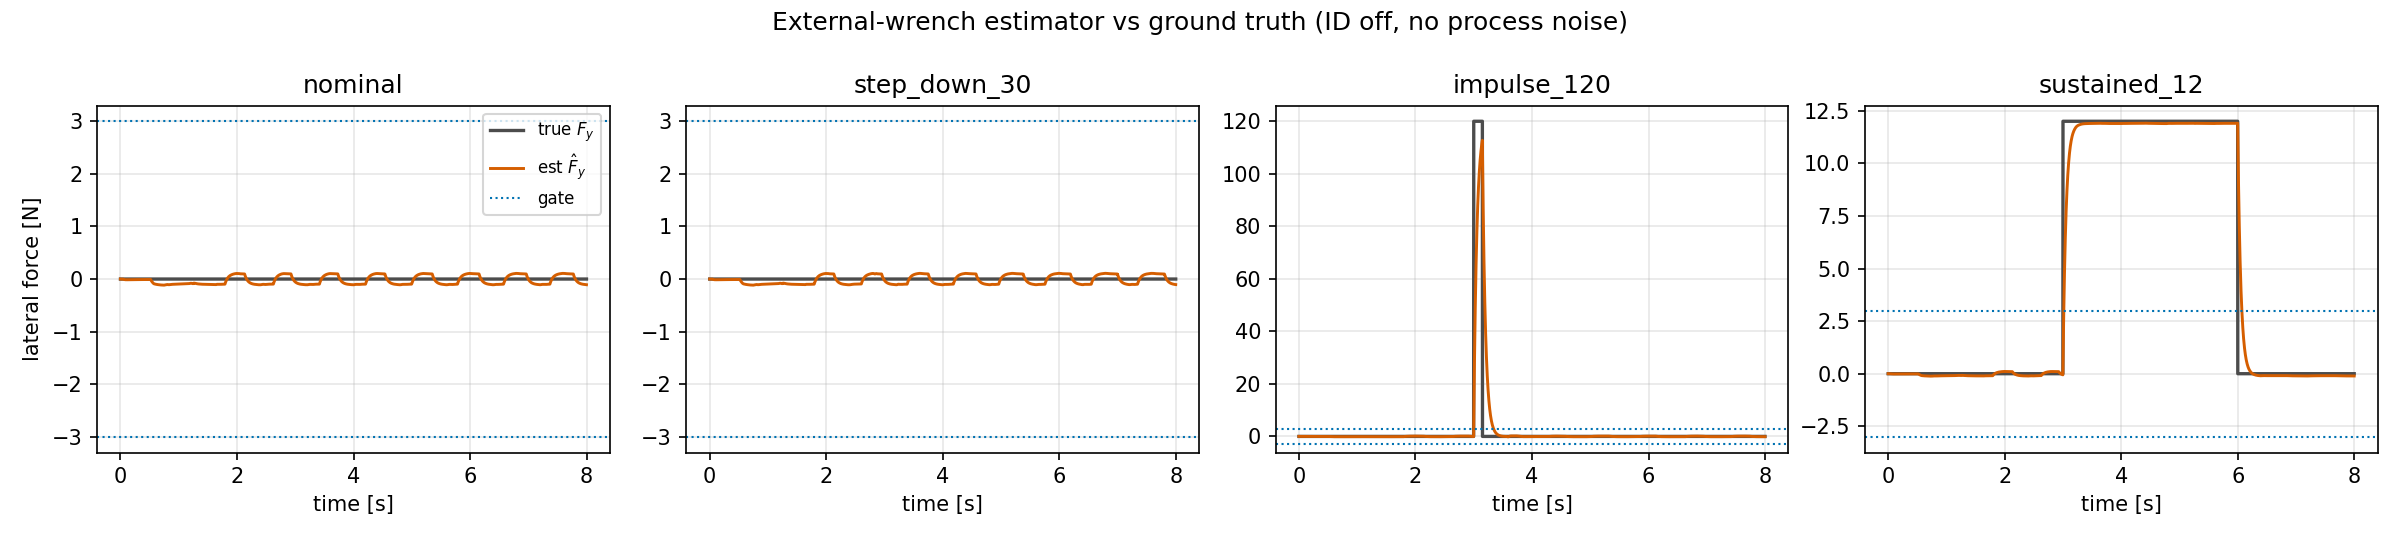
\includegraphics[width=\textwidth]{estimator_validation}
\caption{各测试场景下、关闭交互层时估计的水平外力 $\hat F_{\rm ext}$ 与真实值的对比：在步态与接触切换时没有虚警，冲击检测近乎瞬时且衰减时间约为 $0.19$~s，对持续力的跟踪精度约为 $1$~N。}
\label{fig:estimator}
\end{figure*}

\begin{table}[t]
\caption{外力估计器与真实值对比。}
\label{tab:estimator}
\centering
\begin{tabular}{lrrrr}
\hline
场景 & RMSE & 虚警率 & 检测延迟 & 衰减时间\\
\hline
名义行走 & 0.1 N & 0.0\% & -- & --\\
转向 & 0.1 N & 0.0\% & -- & --\\
对角行走 & 0.1 N & 0.0\% & -- & --\\
台阶下降 30 mm & 0.1 N & 0.0\% & -- & --\\
冲击 120 N & -- & -- & $\le$2 ms & 0.19 s\\
持续 12 N & 1.0 N（跟踪） & -- & 0.01 s & --\\
\hline
\end{tabular}
\end{table}

该估计器不会将触地/离地、步态切换或指令加速度误判为外部交互（虚警率 0\%；所有无外力行走期间残差约为 $0.1$~N），能够近乎瞬时地检测到真实冲击并在 0.19~s 内将其清除，并能将 12~N 的持续力跟踪到 1~N 的精度（表~\ref{tab:estimator}）。\emph{验证中的经验教训：} V1 还捕捉到了一个真实的缺陷——地面反作用力求和中的一个接触力符号错误，导致在箱形地形上估计出的力旋量方向翻转（平地上则是正确的）；正是因为我们把估计值与真实值绘制在一起对比，才发现并修复了这个问题。

\textbf{V2（架构必要性，oracle 消融实验）。} 在相同的瞬态（300~N 单支撑）与持续（8~N）测试上比较六种控制器：策略本身；捕获专用控制器；保持专用控制器；一个仅基于质心运动学的统一控制器（对\emph{偏差}本身而非外力做持续性判断）；力门控控制器；以及一个在扰动起始时刻即以零延迟知晓真实扰动类别的\textbf{oracle} 控制器。

\begin{table}[t]
\caption{Oracle 消融实验：每个专用控制器在其适用范围之外都会失效。}
\label{tab:ablation}
\centering
\begin{tabular}{lrr}
\hline
控制器 & 瞬态跌倒次数 /20 & 持续漂移 (mm)\\
\hline
策略 & 20 & 462\\
捕获专用 & 11 & 1080\\
保持专用 & 20 & 12\\
仅质心统一控制器 & 16 & 719\\
\textbf{力门控} & \textbf{12} & \textbf{13}\\
oracle & 11 & 12\\
\hline
\end{tabular}
\end{table}

每个专用控制器在其适用范围之外都会失效（符号相反的二分法所致）；纯捕获会\emph{放大}持续力（1080~mm，比策略本身还差）。仅基于质心的统一控制器在两项指标上均处于劣势：在所测试的控制器族与扰动协议下，仅依赖质心的仲裁是不够的，而基于外力的持续性判断则能实现接近 oracle 水平的选择（表~\ref{tab:ablation}）。我们并不声称外力信息对\emph{每一种}分类器而言在数学上都是必需的——一个更丰富的时序模型或许能够从上下文中推断出持续时间。力门控控制器在瞬态情形下与 oracle 表现一致，在持续情形下也几乎与之相当。

\textbf{V3（泛化能力，留出集测试）。} 在所有阈值与增益均保持冻结的前提下，我们评估了从未用于调参的情形：留出的冲击\emph{持续时间}（0.10/0.25/0.40~s，相对于设计时使用的 0.15~s）、网格之外的持续力幅值（6/10/14~N）、斜坡上升力，以及间歇性外力。控制器展现出良好的泛化能力：在留出的 0.25~s 持续时间下，其表现与捕获专用控制器相当（正确地将其分类为瞬态，而没有退化为保持模式）；网格之外的持续力幅值也能跟踪其趋势；对一个 1~s 斜坡外力的抑制效果优于裸策略。\textbf{一种失效模式：} 一个快速间歇性外力（0.5~s 开/关）会使持续性判别器失效——间歇性外力本身确实是模糊的（反复推力 vs.\ 一个近似持续的力），置信门与持续性混合机制都会将其保持在一个不稳定的状态。我们将此列为一项局限性（第~\ref{sec:limits}节）。

\textbf{V4（统计显著性）。} 使用 40 个配对的留出种子；瞬态情形通过跌倒次数并配合精确 McNemar 检验来评估，持续情形则通过经地板修正的配对漂移来评估（有外力时的偏移减去同一种子无外力时的偏移，从而抵消步态摇摆/参考相位漂移）。

\begin{table}[t]
\caption{瞬态（上）与持续（下，中位数 [IQR]，单位 mm）。}
\label{tab:stats}
\centering
\setlength{\tabcolsep}{4pt}
\begin{tabular}{lrrrr}
\hline
推力 & 策略跌倒 & 力门控跌倒 & McNemar $p$ & 力门控更差次数\\
\hline
280 N & 24/40 & \textbf{2/40} & $<10^{-4}$ & 0\\
300 N & 40/40 & \textbf{20/40} & $<10^{-4}$ & 0\\
320 N & 40/40 & 36/40 & 0.125 & 0\\
\hline
\end{tabular}

\vspace{4pt}

\begin{tabular}{lrrr}
\hline
外力 & 策略 & 保持专用 & 力门控\\
\hline
8 N & 462 mm & 12 [7--19] & \textbf{13 [8--17]}\\
12 N & 728 mm & 121 [114--132] & 202 [186--218]\\
\hline
\end{tabular}
\end{table}

瞬态情形下的收益具有很强的统计显著性，且在所评估的三个推力幅值下，没有任何一次配对试验变差（表~\ref{tab:stats}）；我们不将“从不变差”这一结论外推到这些条件之外（参见 V3 中的间歇性外力失效情形）。在 8~N 持续力下，本控制器的漂移落在保持专用控制器的分布范围之内（13 [8–17] 对比 12 [7–19]~mm），但我们并不声称二者在形式上等价——配对等价性检验留待未来工作；在 12~N 时，因果检测所带来的代价约为 $1.7$ 倍，幅度不大。该恢复包络（图~\ref{fig:envelope}）显示，在 280~N 之前，本控制器始终将单支撑跌倒率保持在 0\%，而此时策略本身的跌倒率已达 60–87\%。

\textbf{V5（传感鲁棒性）。} 由于估计器要减去实测的接触力，而持续力本身只有 8–12~N，我们对水平方向的足端力偏置 $b_F\in\{-5,-3,0,3,5\}$~N 及测量噪声进行了扫描。名义行走得到了充分保护（在所有偏置和噪声条件下，基座横滚角均为 6.8–6.9$^\circ$），这是因为在线噪声本底会将一个持续性偏置吸收进 $F_{\rm cap}$ 之中：EWMA 会提升 $\sigma_f$，使 $F_{\rm cap}$ 升高到偏置之上，从而捕获始终不会被触发，而持续力的抑制（由偏差驱动、不受门控约束）则不受影响（见补充材料）。持续调节能够容忍 $\pm 5$~N 的偏置（在 $b_F=-5/0/+5$ 时漂移分别为 10/14/22~mm），瞬态方面的收益在较大偏置下会平缓地下降，但仍远优于策略本身。

\textbf{V6（估计器实现方式）。} 在所评估的场景中，有限差分估计器（式~\eqref{eq:fext}）与动量观测器给出的估计结果相当；在虚警率这一指标上，有限差分形式在此处表现更干净，原因是仿真中的质心速度本身已经是干净的。观测器的优势——对\emph{带噪声}速度的鲁棒性——是一个面向硬件的考量。我们将有限差分形式保留为默认实现。

\textbf{捕获放大失效模式。} 仅凭平衡类指标会掩盖一种只有在侧向位置上才能看到的失效：当过程噪声超出死区时，一个未加门控的捕获路径会放大它所介入的、但又无法将其分类为外力的任何漂移，驱动出一个失控的侧向偏移（4~N 噪声下无外力漂移达 1539~mm），且这种情况从不导致跌倒。这是一个控制逻辑问题，而不是调参问题——捕获会朝一个未被分类的漂移方向迈步，从而闭合一个正反馈回路——这正是第一级置信门（第~\ref{sec:gate}节）被设计用来防止的问题，其方式是只有在存在真实交互的置信证据时才启用捕获。加入门控后，无外力漂移降至约 $95$~mm（策略自身的本底水平），同时瞬态与持续方面的收益得以保持或改善（表~\ref{tab:ablation}–\ref{tab:stats}）。在线的、按噪声缩放的阈值（式~\eqref{eq:fcap}）无需手工调参，就能自动恢复出适合特定噪声水平的取值：

\begin{table}[t]
\caption{置信度阈值能够自适应传感噪声（噪声干净时更灵敏，噪声较大时更保守），因此它是一个通用判据，而不是一个针对特定实验调好的常数。}
\label{tab:selfcal}
\centering
\begin{tabular}{rr}
\hline
过程噪声 & 稳定后的 $F_{\rm cap}$\\
\hline
0 N & 1.4 N\\
1 N & 2.1 N\\
4 N & 6.3 N\\
8 N & 10.6 N\\
\hline
\end{tabular}
\end{table}

\section{人形机器人演示}
\label{sec:demo}

在冻结策略之上，该层于行走过程中原位（in-situ）运行。在侧向单支撑推力下，它扩展了恢复包络（图~\ref{fig:envelope}，左）；在侧向持续力下，它将质心保持在名义路径附近，而此时策略本身会出现下垂（图~\ref{fig:envelope}，右）。在地形方面，策略本身已经能够处理的\textbf{台阶下降}不受该层影响，而超过几厘米的盲目\textbf{台阶上升}则会导致所有控制器都出现脚趾绊碰式的\emph{绊倒}——该策略是在平地上训练出来的，无法看到台阶。这并不是交互层的一个弱点：它恰恰说明交互控制无法凭空构造出地形几何信息。一旦感知检测到台阶，规划器就可以抬高或重新定位摆动腿，而交互层则在规划延迟期间维持稳定——二者各自在自己的时间尺度上发挥作用。这正是第~\ref{sec:discussion}节将其转化为一个系统性论证的那个边界。

\begin{figure*}[t]
\centering
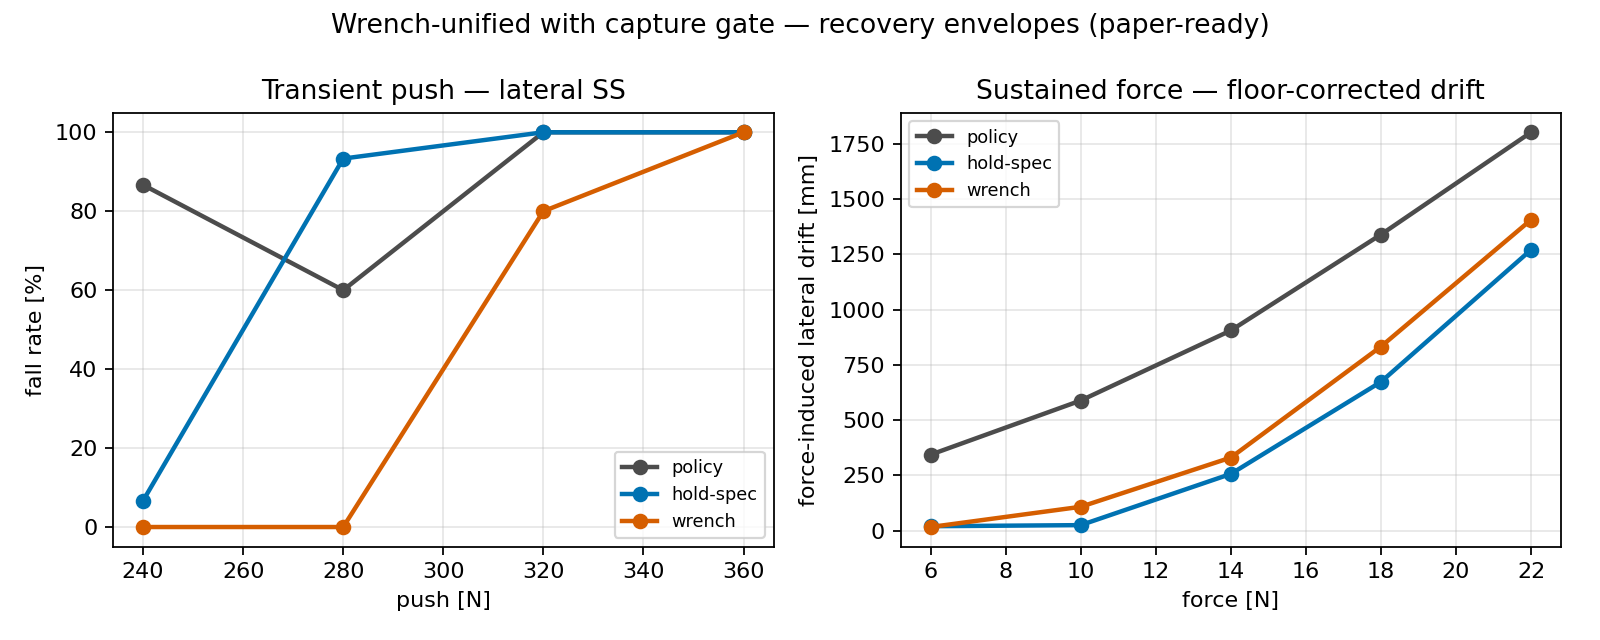
\includegraphics[width=0.7\textwidth]{wrench_envelope_gated}
\caption{恢复包络（置信度门控层与策略本身及保持专用控制器的对比）：(左) 单支撑跌倒率随推力幅值的变化；(右) 经地板修正的稳态侧向漂移随持续力的变化。}
\label{fig:envelope}
\end{figure*}

\section{讨论：基于模型的 Physical AI 层级结构中的交互动力学}
\label{sec:discussion}

本文所提出的层并非意在取代感知或运动规划。它工作在更短的时间尺度上，解决的是一个不同的问题，其最大价值在于作为反应式物理控制与深思熟虑的、基于模型的规划之间的\emph{桥梁}。

\textbf{感知与交互是互补而非竞争的关系。} 感知与世界模型估计的是\emph{世界是什么样子}；运动规划决定的是\emph{接下来该做什么}；而交互动力学掌管的则是\emph{与此同时机器人在物理层面如何进行交互}，即在较慢的循环更新规划期间，基于所估计的交互进行稳定化。盲台阶上升（第~\ref{sec:demo}节）这一例子把这一点讲得很具体：在没有地形感知的情况下，任何交互控制器都无法避免绊倒；但有了地形感知之后，规划器就能抬高或调整落脚点，而该层则在规划延迟期间维持稳定。这里的论断并不是说控制器补偿了感知延迟，而是说交互控制与感知在整个技术栈中占据着不同的、互补的层级。

\textbf{该层能够争取时间。} 对外力而言道理是一样的。一次推力会被立即应对，因为响应只需要 $\hat F_{\rm ext}$。如果扰动超出该层的权限范围，更高层可以拓宽支撑姿态、减速、改变方向、放弃任务，或进入安全模式。所观测到的恢复裕度表明，该层有可能为更慢的规划响应争取额外的时间（延迟的规划器响应本身并未在本文中测试）：
\begin{center}
\emph{外部推力} $\rightarrow$ \emph{交互层}（毫秒级）$\rightarrow$ \emph{机器人得以维持} $\rightarrow$ \emph{规划器}（百毫秒级）$\rightarrow$ \emph{新策略}
\end{center}

\textbf{将交互状态作为规划信号（提议）。} 该层所暴露出的信息，其价值不止于作为一个评估指标。更高层可以消费所估计的外力、其所处模式，以及跌倒速率 $\dot\theta_{\rm fall}$。我们将 $\dot\theta_{\rm fall}$ 视为一种失稳线索，而不是一个经过标定的权限裕度；一个真正的裕度需要综合指令饱和、落脚可达范围与支撑多边形限制等因素，将 $\dot\theta_{\rm fall}$ 与恢复边界相关联留待未来工作。这条向上的路径仅是一个被提议的接口。该层暴露了自身的交互状态，但本文并未将这一回路闭合到规划器，也未对此进行评估。

\textbf{本文贡献在整体框架中的位置。} 在一个基于模型的 Physical AI 技术栈——感知 $\rightarrow$ 规划器 $\rightarrow$ 交互动力学 $\rightarrow$ 全身实现 $\rightarrow$ 机器人——中，本文的贡献是\emph{其中一级}：即规划更新之间的快速物理交互接口。此处的“Physical AI”只是背景语境，而不是本文的结果本身；本文所定义的是这一整体框架中职责明确（估计、对模式进行推理、稳定化）、上下接口清晰的单独一级。

\section{局限性}
\label{sec:limits}

周期接近检测时间尺度的\textbf{间歇性施力}会使持续性判别器失效（V3）；这一情形与门控引入之前的低于阈值的噪声问题，根源是相同的——当该层无法置信地对交互进行分类时，捕获路径就是不安全的。置信门解决了噪声这一情形；间歇性情形则确实是模糊的，仍然是一个开放问题。
在一个学习策略上进行\textbf{全身实现}被发现会使行走失稳（第~\ref{sec:realize}节）；因此交互修正是通过策略的指令接口注入的。在一个基于模型的步行器上，QP 实现方式或许更为可取；本文并未对此作出声称。
\textbf{感知不在本文范围内。} 该层无法凭空构造地形几何信息（盲台阶上升），也无法预判扰动；它提供的是即时稳定化，其权限边界则是留给有能力处理这些问题的层的信号。
本研究仅在一个仿真人形机器人和\textbf{一个步行策略}上进行。该层仅通过其指令接口与策略耦合，因此策略无关性在构造上是成立的；不过，一个跨第二个策略的验证仍将为这一架构性论断提供实证支持，这与其他任务坐标、长距离行走、可变形地面，以及同时进行操作等课题一样，都留待未来工作。

\section{结论}
\label{sec:conclusion}

我们提出了交互动力学（Interaction Dynamics）：一个掌管腿式机器人与世界之间物理交互的快速、短时间尺度的层。它将所有外部交互都表示为一个构型不变的固定模型之上的残差，从质心动量残差中估计外力，并借助一个在线的、按噪声缩放的置信门，以及一个基于持续性、在符号相反的捕获与保持之间进行混合的机制来对其进行推理。该层通过指令接口叠加在一个\emph{冻结}的强化学习策略之上，能够减少推力导致的跌倒（在所测试的推力幅值下没有出现任何配对意义上的性能退化），并将持续力抑制到接近专用控制器的精度，同时名义行走性能不受影响；一个六阶段的验证支持了上述结论，并识别出一种被置信门所解决的捕获放大失效模式。我们提出交互动力学作为感知驱动的规划与全身实现之间的一个候选\emph{快速物理交互层}——它是一个基于模型的 Physical AI 层级结构中的一级，而对该结构的端到端验证仍留待未来工作。

\begin{thebibliography}{19}

\bibitem{r1} Y. Cao and J. Tang, ``Compact Offset-Free Interaction-Error MPC with Applied-Torque Constraints for Physical Human--Robot Interaction,'' 2026, arXiv:2606.08281.

\bibitem{r2} J. Di Carlo, P. M. Wensing, B. Katz, G. Bledt, and S. Kim, ``Dynamic locomotion in the MIT Cheetah 3 through convex model-predictive control,'' in \emph{Proc. IEEE/RSJ IROS}, 2018, pp. 1--9.

\bibitem{r3} D. Kim, J. Di Carlo, B. Katz, G. Bledt, and S. Kim, ``Highly dynamic quadruped locomotion via whole-body impulse control and model predictive control,'' arXiv:1909.06586, 2019.

\bibitem{r4} C. D. Bellicoso, C. Gehring, J. Hwangbo, P. Fankhauser, and M. Hutter, ``Perception-less terrain adaptation through whole body control and hierarchical optimization,'' in \emph{Proc. IEEE-RAS Humanoids}, 2016, pp. 558--564.

\bibitem{r5} T. Koolen \emph{et al.}, ``Design of a momentum-based control framework and application to the humanoid robot Atlas,'' \emph{Int. J. Humanoid Robotics}, vol. 13, no. 1, 2016.

\bibitem{r6} O. Khatib, ``A unified approach for motion and force control of robot manipulators: The operational space formulation,'' \emph{IEEE J. Robotics Autom.}, vol. 3, no. 1, pp. 43--53, 1987.

\bibitem{r7} L. Sentis and O. Khatib, ``Synthesis of whole-body behaviors through hierarchical control of behavioral primitives,'' \emph{Int. J. Humanoid Robotics}, vol. 2, no. 4, pp. 505--518, 2005.

\bibitem{r8} D. E. Orin, A. Goswami, and S.-H. Lee, ``Centroidal dynamics of a humanoid robot,'' \emph{Autonomous Robots}, vol. 35, no. 2--3, pp. 161--176, 2013.

\bibitem{r9} L. Righetti, J. Buchli, M. Mistry, and S. Schaal, ``Inverse dynamics control of floating-base robots with external constraints: A unified view,'' in \emph{Proc. IEEE ICRA}, 2011, pp. 1085--1090.

\bibitem{r10} J.-P. Sleiman, F. Farshidian, M. V. Minniti, and M. Hutter, ``A unified MPC framework for whole-body dynamic locomotion and manipulation,'' \emph{IEEE Robot. Autom. Lett.}, vol. 6, no. 3, pp. 4688--4695, 2021.

\bibitem{r11} N. Hogan, ``Impedance control: An approach to manipulation---Parts I, II, III,'' \emph{ASME J. Dyn. Syst. Meas. Control}, vol. 107, no. 1, pp. 1--24, 1985.

\bibitem{r12} A. Albu-Sch\"{a}ffer, C. Ott, and G. Hirzinger, ``A unified passivity-based control framework for position, torque and impedance control of flexible joint robots,'' \emph{Int. J. Robotics Research}, vol. 26, no. 1, pp. 23--39, 2007.

\bibitem{r13} R. Grandia, F. Jenelten, S. Yang, F. Farshidian, and M. Hutter, ``Perceptive locomotion through nonlinear model-predictive control,'' \emph{IEEE Trans. Robotics}, vol. 39, no. 5, pp. 3402--3421, 2023.

\bibitem{r14} A. De Luca and R. Mattone, ``Sensorless robot collision detection and hybrid force/motion control,'' in \emph{Proc. IEEE ICRA}, 2005, pp. 999--1004.

\bibitem{r15} S. Haddadin, A. De Luca, and A. Albu-Sch\"{a}ffer, ``Robot collisions: A survey on detection, isolation, and identification,'' \emph{IEEE Trans. Robotics}, vol. 33, no. 6, pp. 1292--1312, 2017.

\bibitem{r16} N. Rudin, D. Hoeller, P. Reist, and M. Hutter, ``Learning to walk in minutes using massively parallel deep reinforcement learning,'' in \emph{Proc. Conf. Robot Learning (CoRL)}, 2022, pp. 91--100.

\bibitem{r17} B. Stellato, G. Banjac, P. Goulart, A. Bemporad, and S. Boyd, ``OSQP: An operator splitting solver for quadratic programs,'' \emph{Math. Program. Comput.}, vol. 12, no. 4, pp. 637--672, 2020.

\bibitem{r18} E. Todorov, T. Erez, and Y. Tassa, ``MuJoCo: A physics engine for model-based control,'' in \emph{Proc. IEEE/RSJ IROS}, 2012, pp. 5026--5033.

\bibitem{r19} Y.-Y. Cao, Z. Lin, and D. G. Ward, ``Anti-windup design of output tracking systems subject to actuator saturation and constant disturbances,'' \emph{Automatica}, vol. 40, no. 7, pp. 1221--1228, 2004.

\bibitem{r20} J. Pratt, J. Carff, S. Drakunov, and A. Goswami, ``Capture point: A step toward humanoid push recovery,'' in \emph{Proc. IEEE-RAS Humanoids}, 2006, pp. 200--207.

\bibitem{r21} J. Englsberger, C. Ott, and A. Albu-Sch\"{a}ffer, ``Three-dimensional bipedal walking control based on divergent component of motion,'' \emph{IEEE Trans. Robotics}, vol. 31, no. 2, pp. 355--368, 2015.

\bibitem{r22} B. J. Stephens and C. G. Atkeson, ``Push recovery by stepping for humanoid robots with force controlled joints,'' in \emph{Proc. IEEE-RAS Humanoids}, 2010, pp. 52--59.

\bibitem{r23} T. Johannink \emph{et al.}, ``Residual reinforcement learning for robot control,'' in \emph{Proc. IEEE ICRA}, 2019, pp. 6023--6029.

\bibitem{r24} K. S. Narendra and J. Balakrishnan, ``Adaptive control using multiple models,'' \emph{IEEE Trans. Autom. Control}, vol. 42, no. 2, pp. 171--187, 1997.

\bibitem{r25} J. Vorndamme, M. Schappler, and S. Haddadin, ``Collision detection, isolation and identification for humanoids,'' in \emph{Proc. IEEE ICRA}, 2017, pp. 4754--4761.

\end{thebibliography}

\end{document}
